\documentclass[journal,twoside,web]{ieeecolor}
\usepackage{generic}
\usepackage{cite}
\usepackage{amsmath,amssymb,amsfonts,listings}
\usepackage{algorithmic}
\usepackage[justification=centering]{caption}
\usepackage{float}
\usepackage[dvipsnames]{xcolor}
\usepackage{graphicx}
\usepackage{textcomp}
\usepackage[UTF8]{ctex}
\usepackage[colorlinks, linkcolor=blue, urlcolor=red]{hyperref}
\setCJKfamilyfont{myfont}{msyhbd.ttc}
\newcommand{\SetFont}{\CJKfamily{myfont}}
%\SetFont{生僻字}
\def\BibTeX{{\rm B\kern-.05em{\sc i\kern-.025em b}\kern-.08em
    T\kern-.1667em\lower.7ex\hbox{E}\kern-.125emX}}
\markboth{智能工程学院  智能科学与技术}
{人工智能编程语言大作业}
\lstset{
    language=Python,
    basicstyle=\ttfamily\small,
    keywordstyle=\bfseries\color{NavyBlue},
    commentstyle=\itshape\color{red!50!green!50!blue!50},
    stringstyle=\bfseries\color{PineGreen!90!black},
    emph={self}, 
    emphstyle=\bfseries\color{Rhodamine},
    backgroundcolor=\color{black!3},
    frame=shadowbox,
    frameround=fttt,
    numbers=left,
    numberstyle=\tiny,
    stepnumber=1,
    numbersep=5pt,
    breaklines=true,
    columns=flexible,
    xleftmargin=3em,
    xrightmargin=0em,
    aboveskip=1em,
    framexleftmargin=1em,
    escapeinside=``,
}

\begin{document}
\title{人工智能编程语言大作业}
\author{陈海弘,方唯特
\thanks{陈海弘,23354049,(e-mail: chenhh93@mail2.sysu.edu.cn),}
\thanks{方唯特,23354057,(e-mail: fangwt5@mail2.sysu.edu.cn)。}
}

\maketitle

\begin{abstract}
    本文主要介绍了进化算法的基本原理,以及如何使用Python和Matlab实现投资问题的代码。在投资问题中,我们需要根据股票的成本价和收益率,选择最佳的投资组合。通过进化算法的交叉和变异操作,可以生成新的个体,并对其进行处理。最后,我们展示了交叉和变异操作的具体实现,以及输出结果的分析。
\end{abstract}

\begin{IEEEkeywords}
    进化算法,投资问题,Python,Matlab
\end{IEEEkeywords}
\section{第一题:进化算法基本原理}
    进化算法是一种基于随机搜索的优化方法,主要包括以下步骤:

	1.	种群初始化:随机生成一个包含$P_0$个个体的初始种群。

	2.	交叉操作:以概率$p_c$在种群中进行交叉,生成新个体,增加种群规模至$P$。

	3.	变异操作:以概率$p_m$在种群中执行变异,调整个体基因。

	4.	选择操作:选择优质个体进入下一代,保持种群规模为$P_0$。

	5.	终止条件:当达到预定代数$Gen$时输出最优个体,否则重复步骤2。

 流程图展示:
\begin{figure}[H]
    \hspace{3cm}
    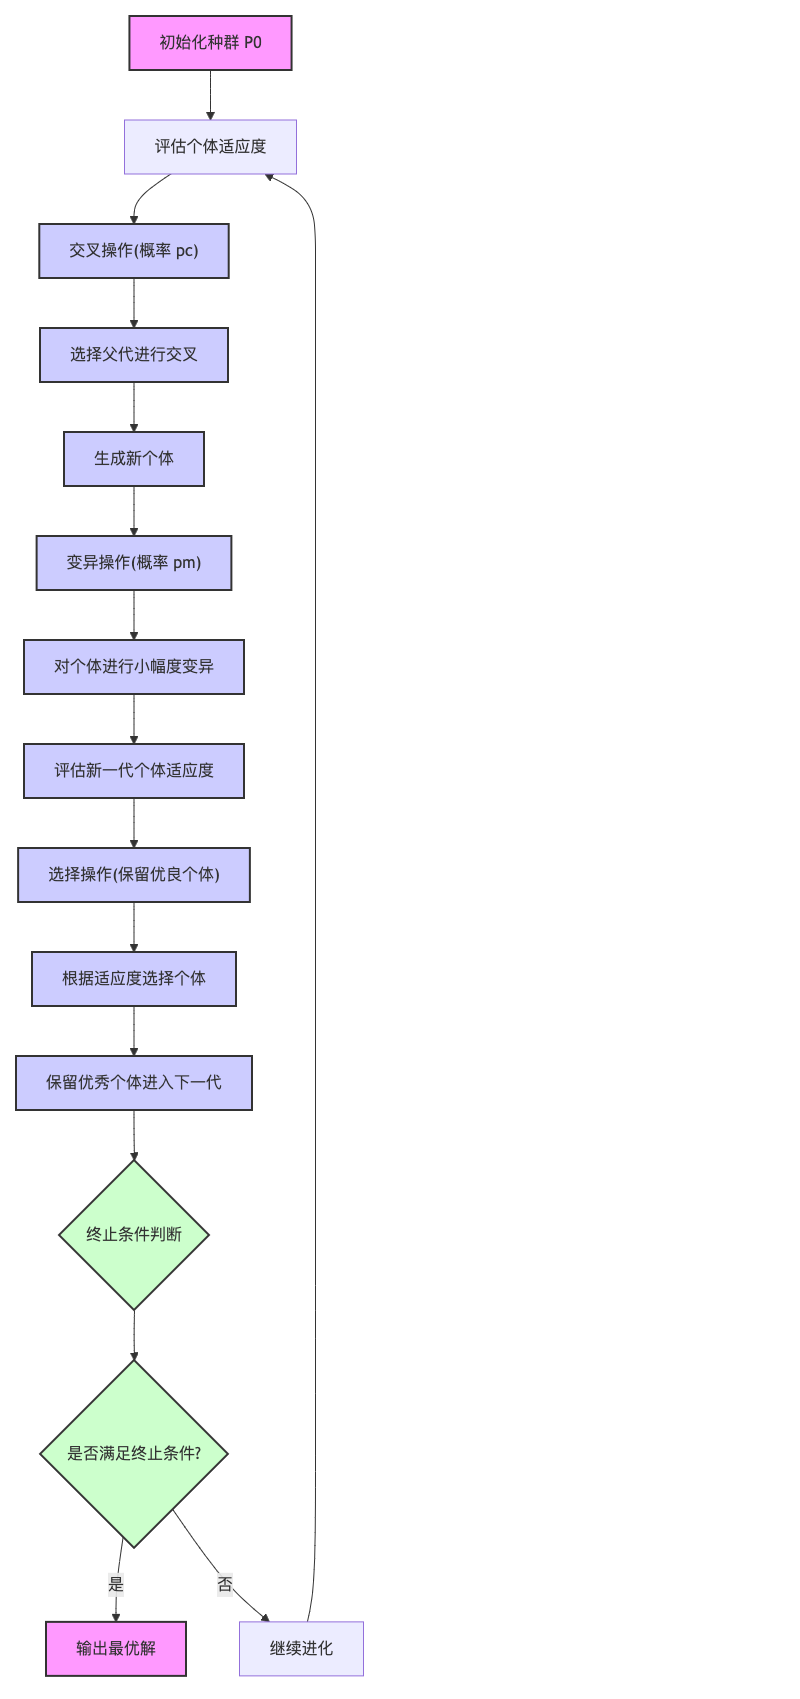
\includegraphics[width=0.45\textwidth]{img/graph.png}
    \caption{进化算法流程图}
\end{figure}

\section{第二题:代码实现投资问题}
假如你是一名投资者,打算投资中国股市,现在需要决定选择哪些股票进行投资。为了简化模型,设最大可用于投资的金额为700元,每种股票最多购买1股。(实际投资中,每种股票的最少需要购买1手,也就是100股,此处仅为了简化问题。)

现收集到2024年1月到2024年9月时间段内中国A股排名前100(实际有效数据为96只股票)的股票的信息,包括股票名称、最新价(单位:/股,2024年9月数据)、成本价(单位:/股,2024年1月数据)和收益率(100\%)。你希望通过这些信息,分析2024年1月时如何投资能够获得更高的收益,以此作为未来投资的参考。
\subsection{Python}
\begin{enumerate}
    \item \textbf{获取股票数据}:首先,通过Akshare库的接口获取A股市场的股票数据。使用函数 \texttt{stock\_zh\_a\_spot\_em()} 获取实时股票信息,包括股票的最新价格、市值等数据。
    
    \item \textbf{数据排序与筛选}:将获取到的股票数据按总市值进行排序,筛选出市值排名前100的公司,并将结果保存为CSV文件。这一步的目的是找到市值最大的前100只股票,以便后续的处理。
    
    \item \textbf{数据清理与计算成本价}:读取保存的CSV文件,并删除缺少最新价格的股票数据。然后,基于每只股票的最新价格和年初至今的涨跌幅,计算其“成本价”。成本价的计算公式为:
    \[
    \text{成本价} = \frac{\text{最新价}}{1 + \frac{\text{年初至今涨跌幅}}{100}}
    \]
    计算结果将新增为一列“成本价”,并将处理后的数据保存为新的CSV文件。
    
    \item \textbf{股票排序与编码生成}:加载处理后的数据,按成本价降序排序,选出成本价最高的前10只股票。接着,构建一个长度为96的编码数组,其中前10只股票的编码为1,其余为0。这个编码数组可以用于后续的股票筛选或机器学习任务中。
    
    \item \textbf{结果输出与验证}:最后,输出生成的编码数组,验证编码是否正确。输出的编码数组会包含前10只股票的位置设置为1,其他位置为0。
\end{enumerate}

Python代码如下:
\begin{lstlisting}
    # akshare是一个用于获取股票市场的包,可进行简单的排序等操作
    import akshare as ak
    import pandas as pd
    '''
        该代码用于获取并处理股票信息,供同学们参考
        处理后的股票数据文件已给出,名为“Top96_A_Lite”,格式为CSV文件
        由于股票市场变动频繁,为保证统一,请同学们统一提供的“Top96_A_Lite”文件。
    '''
    
    # 获得A股股票信息
    stock_zh_a_spot_df = ak.stock_zh_a_spot_em()
    # 按照总市值排序,获得Top100排行榜
    stock_zh_a_spot_df_sorted = stock_zh_a_spot_df.sort_values(by="总市值", ascending=False)
    top_100_market_value = stock_zh_a_spot_df_sorted.head(100)
    # 查询市值Top 100的公司
    top_100_market_value.to_csv("Top100_A")
    
    file_path = 'Top100_A'
    data = pd.read_csv(file_path, usecols=['代码', '名称', '最新价', '年初至今涨跌幅'])
    # 删除满足特定查询条件的行
    # 删除满足某条件的所有行
    # 直接在原DataFrame上操作
    data.dropna(subset=['最新价'], axis=0, inplace=True)
    data['成本价'] = data['最新价'] / (1 + data['年初至今涨跌幅'] / 100)
    data.to_csv('Top'+ str(len(data)) + '_A_Lite', index=False)
    
    import pandas as pd
    
    # 假设已加载数据,文件名为 'Top96_A_Lite.csv'
    data = pd.read_csv('Top96_A_Lite.csv')
    print(data)
    
    # 按成本价降序排序,并获取前10只股票
    top_10_stocks = data.sort_values(by='成本价', ascending=False).head(10)
    
    # 构造编码数组:长度为96(所有股票数),对前10只股票设置为1,其余为0
    n_stocks = len(data)
    encoding = [0] * n_stocks
    
    # 找到前10只股票的索引,并将对应位置的编码设置为1
    for index in top_10_stocks.index:
        encoding[index] = 1
    
    print("编码结果:", encoding)
    
    print([0, 0, 0, 1, 0, 0, 0, 0, 0, 1, 0, 0, 0, 0, 1, 0, 0, 0, 0, 1, 0, 0, 0, 0, 0, 0, 0, 1, 0, 0, 0, 0, 0, 0, 0, 0, 0, 0, 0, 0, 0, 0, 1, 0, 0, 0, 0, 1, 0, 0, 0, 0, 0, 0, 0, 0, 0, 1, 1, 0, 0, 0, 0, 0, 0, 0, 0, 0, 0, 0, 0, 0, 0, 0, 0, 0, 0, 0, 0, 1, 0, 0, 0, 0, 0, 0, 0, 0, 0, 0, 0, 0, 0, 0, 0, 0]
          == [0, 0, 0, 1, 0, 0, 0, 0, 0, 1, 0, 0, 0, 0, 1, 0, 0, 0, 0, 1, 0, 0, 0, 0, 0, 0, 0, 1, 0, 0, 0, 0, 0, 0, 0, 0, 0, 0, 0, 0, 0, 0, 1, 0, 0, 0, 0, 1, 0, 0, 0, 0, 0, 0, 0, 0, 0, 1, 1, 0, 0, 0, 0, 0, 0, 0, 0, 0, 0, 0, 0, 0, 0, 0, 0, 0, 0, 0, 0, 1, 0, 0, 0, 0, 0, 0, 0, 0, 0, 0, 0, 0, 0, 0, 0, 0])
    
\end{lstlisting}
\subsection{Matlab}
\begin{enumerate}
    \item \textbf{读取股票数据:} 
    使用 \texttt{detectImportOptions} 和 \texttt{readtable} 函数读取存储在 \texttt{Top96\_A\_Lite.csv} 文件中的股票数据。通过设置选项 \texttt{VariableNamingRule = 'preserve'},保留了数据表中的原始列标题。读取的数据包括股票的代码、名称、最新价格、年初至今的涨跌幅和成本价格。

    \item \textbf{提取股票信息:} 
    从数据表中提取出相关股票信息,包括股票数量(\texttt{stock\_num})、股票代码(\texttt{stock\_codes})、股票名称(\texttt{stock\_names})、最新价格(\texttt{latest\_prices})、收益率(\texttt{profit\_rates})以及成本价格(\texttt{cost\_prices})。这些信息将用于后续的选择操作。

    \item \textbf{选择成本价格最高的前10支股票:} 
    使用 \texttt{sort} 函数对成本价格(\texttt{cost\_prices})进行降序排序,并获得排序后的索引(\texttt{cost\_sorted\_idx})。接下来,初始化一个零向量 \texttt{top10\_stock\_codes},其长度与股票数量相同。通过将排序后的前10个索引位置的元素设置为1,表示选择了成本价格最高的10支股票。最终,输出这些股票的编码向量。

    \item \textbf{输出:} 
    使用 \texttt{disp} 函数将编码向量 \texttt{top10\_stock\_codes} 输出,展示选择的成本价格最高的10支股票。
\end{enumerate}

Matlab代码如下:
\begin{lstlisting}
    clc;
    clear;
    
    % 读取股票数据
    opts = detectImportOptions('Top96_A_Lite.csv');  % 检测导入选项
    opts.VariableNamingRule = 'preserve';            % 保留原始列标题
    data = readtable('Top96_A_Lite.csv', opts);      % 读取数据
    
    % 提取股票信息
    stock_num = size(data, 1);                       % 获取股票数量
    stock_codes = data.("代码");                     % 股票代码
    stock_names = data.("名称");                     % 股票名称
    latest_prices = data.("最新价");                  % 最新价
    profit_rates = data.("年初至今涨跌幅");          % 收益率
    cost_prices = data.("成本价");                   % 成本价
    
    
    
    
    
    % 题目2:选择成本价格最高的前 10 支股票的编码
    [~, cost_sorted_idx] = sort(cost_prices, 'descend'); % 按成本价降序排序
    top10_stock_codes = zeros(stock_num, 1);              % 初始化编码向量
    top10_stock_codes(cost_sorted_idx(1:10)) = 1;         % 将前10支股票标记为1
    fprintf('选择成本价最高的10支股票的编码为:\n');
    disp(top10_stock_codes);
\end{lstlisting}
\subsubsection*{总之}

\section{第三题:交叉操作实现}
\subsection{Python}
本段代码的核心思路是通过模拟进化算法中的交叉和变异操作来生成新的个体,并对其进行处理。具体步骤如下:

\begin{enumerate}
    \item \textbf{数据准备}:首先,从数据中提取出每只股票的成本价格(\texttt{cost\_prices})和收益率(\texttt{returns})数据。为了选择特定的股票,首先根据成本价格和收益率进行排序,选择出最高成本价格和最低收益率的前30只股票。
    
    \item \textbf{编码表示}:在选择出成本价格最高的前30只股票和收益率最低的前30只股票后,使用0和1的编码方式进行表示。对于选中的股票,编码为1,未选中的股票编码为0。使用Numpy的 \texttt{argsort} 方法对股票进行排序,并根据排序结果为股票编码。
    
    \item \textbf{交叉操作}:在交叉操作中,首先随机选择一个交叉点(不包括开头和结尾),然后将两个个体(\texttt{x1} 和 \texttt{x2})在交叉点前后的部分进行交换。通过 \texttt{np.concatenate} 实现两个个体的交叉,生成新的个体(\texttt{x1\_new} 和 \texttt{x2\_new})。交叉的目的是结合两个父代个体的优点,从而生成更好的后代个体。
    
    \item \textbf{变异操作}:在变异操作中,使用指定的变异率(10\%)对新生成的个体进行变异。通过遍历个体的每一个基因(即股票的编码),以给定的概率将该基因从0变为1,或者从1变为0。这一过程通过 \texttt{mutate} 函数实现,目的是增加种群的多样性,防止陷入局部最优解。
    
    \item \textbf{输出结果}:输出交叉前后的个体编码、交叉点的位置,以及变异前后的个体编码。通过这些输出可以观察到交叉和变异操作对个体的具体影响,进而评估操作是否符合预期。
\end{enumerate}

Python代码如下:
\begin{lstlisting}

    import numpy as np

    # 生成示例数据(问题2中的成本价格和收益率数据)
    cost_prices = data['成本价'].values
    returns = data['年初至今涨跌幅'].values      # 收益率(百分比)
    
    # 选择成本价格最高的前30种股票
    highest_cost_indices = np.argsort(-cost_prices)[:30]
    x1 = np.zeros(len(cost_prices), dtype=int)
    x1[highest_cost_indices] = 1  # 设置编码
    
    # 选择收益率最低的前30种股票
    lowest_return_indices = np.argsort(returns)[:30]
    x2 = np.zeros(len(returns), dtype=int)
    x2[lowest_return_indices] = 1  # 设置编码
    
    # 随机选择交叉点并进行交叉操作
    crossover_point = np.random.randint(1, len(cost_prices))  # 交叉点(不包括开头和结尾)
    x1_new = np.concatenate([x1[:crossover_point], x2[crossover_point:]])
    x2_new = np.concatenate([x2[:crossover_point], x1[crossover_point:]])
    
    # 输出结果
    print("原始 x1:", x1)
    print("原始 x2:", x2)
    print("交叉点位置:", crossover_point)
    print("新 x1:", x1_new)
    print("新 x2:", x2_new)
    
    import numpy as np
    
    # 确定变异位数(10%)
    mutation_rate = 0.1
    
    # 定义变异操作
    def mutate(individual, mutation_rate):
        for i in range(len(individual)):
            if np.random.rand() < mutation_rate:
                individual[i] = 1 - individual[i]  # 0变为1,1变为0
        return individual
    
    # 对新生成的解进行变异操作
    x1_mutated = mutate(x1_new.copy(), mutation_rate)
    x2_mutated = mutate(x2_new.copy(), mutation_rate)
    
    # 输出结果
    print("变异前 x1_new:", x1_new)
    print("变异后 x1_mutated:", x1_mutated)
    print("变异前 x2_new:", x2_new)
    print("变异后 x2_mutated:", x2_mutated)
    
    #Gen 最大迭代次数  pc 交叉概率  pm 变异概率  p0 初始种群  p 种群
\end{lstlisting}
\subsection{Matlab}
\begin{enumerate}
    \item \textbf{交叉操作前的编码:} 
    首先,代码按照收益率(\texttt{profit\_rates})升序对股票进行排序,使用 \texttt{sort} 函数获取排序后的索引(\texttt{profit\_sorted\_idx})。接着,定义了两个零向量 \texttt{x1} 和 \texttt{x2},长度与股票数量相同。 \texttt{x1} 对应前30支成本价格最高的股票,\texttt{x2} 对应前30支收益率最低的股票,通过索引将相应位置的元素设置为1。最终,输出交叉之前的两个编码向量 \texttt{x1} 和 \texttt{x2}。

    \item \textbf{交叉函数定义:} 
    交叉操作模拟了遗传算法中的基因交叉过程。首先,检查两个个体的长度是否相同。如果不相同,则抛出错误。然后,确保 \texttt{x1} 和 \texttt{x2} 都是行向量。通过随机选择一个交叉点,代码将两个编码向量在交叉点进行交换,生成新的编码向量 \texttt{new\_x1} 和 \texttt{new\_x2}。最后,输出交叉点的位置以及交叉后的新编码向量。

    \item \textbf{变异函数定义:} 
    定义了一个变异函数 \texttt{mutate0},该函数模拟基因突变的过程。根据设定的变异率 \texttt{mutation\_rate},遍历每个基因,如果随机生成的数小于变异率,则反转基因(0变为1,1变为0)。变异操作完成后,返回变异后的个体。

    \item \textbf{调用交叉与变异:} 
    在交叉函数执行后,调用变异函数对新的编码向量进行变异。最终,输出变异后的编码向量。
\end{enumerate}

Matlab代码如下:
\begin{lstlisting}
    % 题目3:交叉操作
    [~, profit_sorted_idx] = sort(profit_rates);       % 按收益率升序排序
    x1 = zeros(stock_num, 1);
    x1(cost_sorted_idx(1:30)) = 1;                      % 前30支成本价最高的股票
    x2 = zeros(stock_num, 1);
    x2(profit_sorted_idx(1:30)) = 1;                    % 前30支收益率最低的股票
    
    fprintf('交叉之前的x1和x2编码:\n');
    disp('x1:');
    disp(x1);
    disp('x2:');
    disp(x2);
    
    % 定义交叉函数
    function [new_x1, new_x2, crossover_point] = crossover(x1, x2)
        % 确保两个个体的长度相同
        if length(x1) ~= length(x2)
            error('两个个体的长度不相同');
        end
        
        % 强制将x1和x2转换为行向量
        x1 = reshape(x1, 1, []);  % 转换为行向量
        x2 = reshape(x2, 1, []);  % 转换为行向量
    
        % 输出调试信息,查看x1和x2的长度
        disp(['x1长度: ', num2str(length(x1))]);
        disp(['x2长度: ', num2str(length(x2))]);
        
        % 随机选择一个交叉点
        crossover_point = randi([1, length(x1)-1]);  % 随机选择一个交叉点,保证不越界
        
        % 进行交叉操作
        new_x1 = [x1(1:crossover_point), x2(crossover_point+1:end)];
        new_x2 = [x2(1:crossover_point), x1(crossover_point+1:end)];
        
        % 输出交叉后的结果
        disp('new_x1:');
        disp(new_x1);
        disp('new_x2:');
        disp(new_x2);
    end
    
    % 调用交叉函数进行交叉操作
    [new_x1, new_x2, crossover_point] = crossover(x1, x2);
    fprintf('交叉操作发生的位置: %d\n', crossover_point);
    fprintf('交叉后的x1和x2编码:\n');
    disp('new_x1:');
    disp(new_x1);
    disp('new_x2:');
    disp(new_x2);
    
    % 定义变异函数
    function mutated_individual = mutate0(individual, mutation_rate)
        % 遍历每个基因
        for i = 1:length(individual)
            % 根据变异率决定是否变异
            if rand() < mutation_rate
                individual(i) = 1 - individual(i);  % 反转基因(0变1,1变0)
            end
        end
        % 返回变异后的个体a
        mutated_individual = individual;
    end
\end{lstlisting}
\section{第四题:变异操作实现}
所谓变异操作即为随机改变某个个体的部分编码,达到一个局部搜索的目的,例如:
x1 = 1 0 1 0 1 0 0 0 1
对最后一位进行变异,结果为:
x1’ = 1 0 1 0 1 0 0 0 0

\subsection{Python}
\begin{enumerate}
    \item \textbf{输入参数}:包含多个个体的种群 $P$ 和变异概率 $p_m$。变异概率决定了每个位翻转的可能性。
    \item \textbf{逐个处理个体}:遍历种群中的每个个体 $I$,对其基因序列中的每个位进行检查。
    \item \textbf{判断是否变异}:对每个位生成一个随机数 $rand(0, 1)$,如果该随机数小于变异概率 $p_m$,则执行变异操作。
    \item \textbf{执行变异操作}:将基因位的值翻转,即从 $0$ 变为 $1$ 或从 $1$ 变为 $0$。
    \item \textbf{输出结果}:返回所有个体变异后的新种群 $P'$。
\end{enumerate}

Python代码如下:
\begin{lstlisting}
    # 变异操作
    def mutation(population, pm):
        for individual in population:
            for i in range(len(individual)):
                if np.random.rand() < pm:
                    individual[i] = 1 - individual[i]
        return population
\end{lstlisting}

\subsection{Matlab}
\begin{enumerate}
    \item \textbf{变异操作函数设计}:  
    变异函数以染色体为输入,通过概率判断是否对基因位进行翻转,提升种群的多样性。实现步骤包括:
    \begin{itemize}
        \item 复制输入染色体,避免直接修改原数据。
        \item 遍历每个位,基于随机数与变异概率的比较决定是否翻转。
    \end{itemize}

    \item \textbf{初始染色体生成}:  
    根据投资组合的优化需求,定义两种初始编码方式:
    \begin{itemize}
        \item \textbf{成本价最高编码}:提取成本价最高的前 30 支股票,将对应位置设置为 1。
        \item \textbf{收益率最低编码}:依据年初涨跌幅排序,提取收益率最低的前 30 支股票,同样以二进制编码方式表示。
    \end{itemize}

    \item \textbf{交叉操作}:  
    对两组初始染色体进行交叉操作,生成下一代后代染色体,从而实现信息的组合与重组。

    \item \textbf{变异处理}:  
    对交叉操作后生成的第一代后代染色体执行变异,以概率 $0.01$ 翻转部分基因位,确保优化过程的多样性和探索能力。

    \item \textbf{编码结果打印与分析}:  
    逐步打印以下编码结果,方便观察优化过程和结果对比:
    \begin{itemize}
        \item 初始编码(成本价前 10)。
        \item 成本价前 30 的编码结果。
        \item 收益率最低前 30 的编码结果。
        \item 交叉操作后的编码结果。
        \item 变异操作后的最终编码。
    \end{itemize}
\end{enumerate}
Matlab代码如下:
\begin{lstlisting}
    % 变异操作函数
    function mutated_chromosome = mutation_function(chromosome, mutation_probability)
        % 复制染色体
        mutated_chromosome = chromosome;
        % 进行变异
        for j = 1:length(mutated_chromosome)
            if rand < mutation_probability
                mutated_chromosome(j) = 1 - mutated_chromosome(j);
            end
        end
    end
    
    % 获取成本价最高的前30只股票
    top_30_cost_indices = sorted_by_cost(1:30);
    chromosome1 = zeros(1, height(stock_data));
    chromosome1(top_30_cost_indices) = 1;
    
    % 根据年初涨跌幅排序,提取收益率最低的30只股票
    [~, sorted_by_return] = sort(stock_data.("年初涨跌幅"), 'ascend');
    bottom_30_return_indices = sorted_by_return(1:30);
    chromosome2 = zeros(1, height(stock_data));
    chromosome2(bottom_30_return_indices) = 1;
    
    % 执行交叉操作
    [offspring1, offspring2] = crossover_function(chromosome1, chromosome2);
    
    % 对其中一个后代染色体进行变异
    mutated_offspring1 = mutation_function(offspring1, 0.01);
    
    % 打印编码结果
    disp('初始编码(成本价前10):');
    disp(stock_encoding);
    disp('编码1(成本价前30):');
    disp(chromosome1);
    disp('编码2(收益率最低前30):');
    disp(chromosome2);
    disp('交叉后编码1:');
    disp(offspring1);
    disp('变异后的编码1:');
    disp(mutated_offspring1);
    
\end{lstlisting}
\section{第五题:进化操作实现}
\subsection{Python}
\begin{enumerate}
    \item \textbf{运行遗传算法:}
    \begin{itemize}
        \item 初始化一个字典 \texttt{results},用于存储每个参数集的最佳适应度和平均适应度。
        \item 参数集 \texttt{params} 包含了多个遗传算法的参数组合,包括:
        \begin{itemize}
            \item \texttt{Gen}:遗传算法的代数(代数的数量)。
            \item \texttt{pc}:交叉概率。
            \item \texttt{pm}:变异概率。
            \item \texttt{P0}:初始种群。
            \item \texttt{P}:种群大小。
        \end{itemize}
        \item 对于每一组参数,通过调用 \texttt{genetic\_algorithm} 函数来执行遗传算法,并返回每一代的最佳适应度(\texttt{best})和平均适应度(\texttt{avg})。
    \end{itemize}
    
    \item \textbf{绘制结果:}
    \begin{itemize}
        \item 使用 \texttt{matplotlib} 库绘制每个参数集的适应度变化曲线。每个图像展示了“最佳适应度”和“平均适应度”随代数的变化。
        \item 通过 \texttt{plt.subplot} 在一个 2x3 网格中绘制多幅子图,展示每个参数集的遗传算法结果。
        \item 每幅图标注标题、x 轴(表示代数)和 y 轴(表示适应度),并添加图例。
        \item 使用 \texttt{plt.tight\_layout()} 调整图形布局,使其不会重叠,并通过 \texttt{plt.show()} 展示最终的图形。
    \end{itemize}
\end{enumerate}
\begin{enumerate}

    \item \textbf{参数定义与初始化}:
    \begin{itemize}
        \item 输入参数包括代数 $Gen$、交叉概率 $pc$、变异概率 $pm$、初始种群大小 $P0$、精英数量 $P$ 和种群初始化方法。
        \item 根据初始方法(例如随机初始化),生成 $P0$ 个染色体,每个染色体的长度与股票数量一致。
        \item 定义两个列表:\texttt{best\_solutions} 用于记录每一代的最佳适应度值,\texttt{average\_fitness} 用于记录每一代的平均适应度值。
    \end{itemize}

    \item \textbf{遗传循环}:
    算法通过循环 $Gen$ 代来模拟种群进化,单代进化的主要步骤如下:
    \begin{enumerate}
        \item \textbf{适应度计算}:
        \begin{itemize}
            \item 使用适应度函数 \texttt{fitness},基于输入的股票成本、收益率和投资上限,计算当前种群中每个个体的适应度值。
            \item 记录当前代中最大适应度值和平均适应度值,分别存储于 \texttt{best\_solutions} 和 \texttt{average\_fitness} 列表中。
        \end{itemize}

        \item \textbf{精英保留策略}:
        \begin{itemize}
            \item 按适应度值从高到低排序,保留 $P$ 个适应度最高的个体作为精英个体,确保最优解不会被丢失。
        \end{itemize}

        \item \textbf{选择操作}:
        \begin{itemize}
            \item 采用轮盘赌选择法(\texttt{roulette\_wheel\_selection}),根据适应度比例随机选择个体,生成新的种群。
        \end{itemize}

        \item \textbf{交叉操作}:
        \begin{itemize}
            \item 对选择后的种群进行交叉操作(\texttt{crossover}),以交叉概率 $pc$ 为条件,结合多个染色体的信息生成新个体。
        \end{itemize}

        \item \textbf{变异操作}:
        \begin{itemize}
            \item 对交叉后的种群进行变异操作(\texttt{mutation}),以变异概率 $pm$ 随机翻转基因位,增加种群的多样性。
        \end{itemize}

        \item \textbf{更新种群}:
        \begin{itemize}
            \item 将精英个体与变异后的新种群组合,形成下一代的种群。
        \end{itemize}
    \end{enumerate}

    \item \textbf{参数调试与运行}:
    \begin{itemize}
        \item 定义多组参数组合,每组包含代数、交叉概率、变异概率、初始种群大小及精英数量。
        \item 遍历参数集,调用主函数运行遗传算法,记录每组参数的最佳适应度和平均适应度变化趋势。
    \end{itemize}

    \item \textbf{结果可视化}:
    \begin{itemize}
        \item 为每组参数绘制适应度变化图,包括最佳适应度曲线和平均适应度曲线,便于观察不同参数设置的优化效果。
        \item 使用多子图展示,图形横坐标为代数,纵坐标为适应度值,图例区分两种曲线。
    \end{itemize}

\end{enumerate}
Python代码如下:
\begin{lstlisting}
    # 遗传算法主函数
    def genetic_algorithm(Gen, pc, pm, P0, P, initialization_method="random"):
        n_stocks = len(cost_prices)
        population = initialize_population(initialization_method, P0, n_stocks)
        best_solutions = []
        average_fitness = []
    
        for generation in range(Gen):
            # 计算适应度
            fitness_values = fitness(population, cost_prices, returns, max_investment)
            best_solutions.append(fitness_values.max())
            average_fitness.append(fitness_values.mean())
    
            # 精英保留:保留 P 个最优个体
            elite_indices = fitness_values.argsort()[-P:]
            elites = population[elite_indices]
    
            # 选择、交叉和变异操作
            selected_population = roulette_wheel_selection(population, fitness_values)
            crossed_population = crossover(selected_population, pc)
            mutated_population = mutation(crossed_population, pm)
    
            # 将精英加入下一代
            population = np.vstack((elites, mutated_population[:P0 - P]))
    
        return best_solutions, average_fitness
    
    # 参数集合
    params = [
        (100, 0.1, 0.01, 10, 15),
        (200, 0.3, 0.01, 10, 15),
        (200, 0.15, 0.01, 10, 15),
        (200, 0.1, 0.02, 10, 15),
        (200, 0.2, 0.02, 20, 30),
        (200, 0.2, 0.02, 6, 8),
    ]
    # 运行遗传算法
    results = {}
    for i, (Gen, pc, pm, P0, P) in enumerate(params):
        best, avg = genetic_algorithm(Gen, pc, pm, P0, P, initialization_method="random")
        results[f"ParamSet {i+1}"] = (best, avg)
    
    # 绘制结果
    plt.figure(figsize=(12, 8))
    for i, (key, (best, avg)) in enumerate(results.items()):
        plt.subplot(2, 3, i+1)
        plt.plot(best, label='Best Fitness')
        plt.plot(avg, label='Average Fitness')
        plt.title(key)
        plt.xlabel('Generation')
        plt.ylabel('Fitness')
        plt.legend()
    plt.tight_layout()
    plt.show()
    
\end{lstlisting}

\begin{figure}
    \centering
    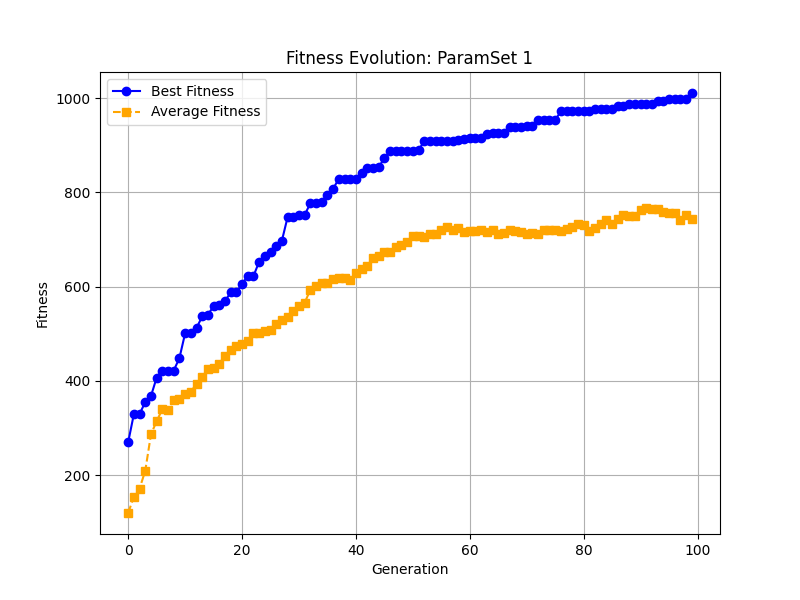
\includegraphics[width=0.3\textwidth]{img/Figure_1.png}
    \centering
    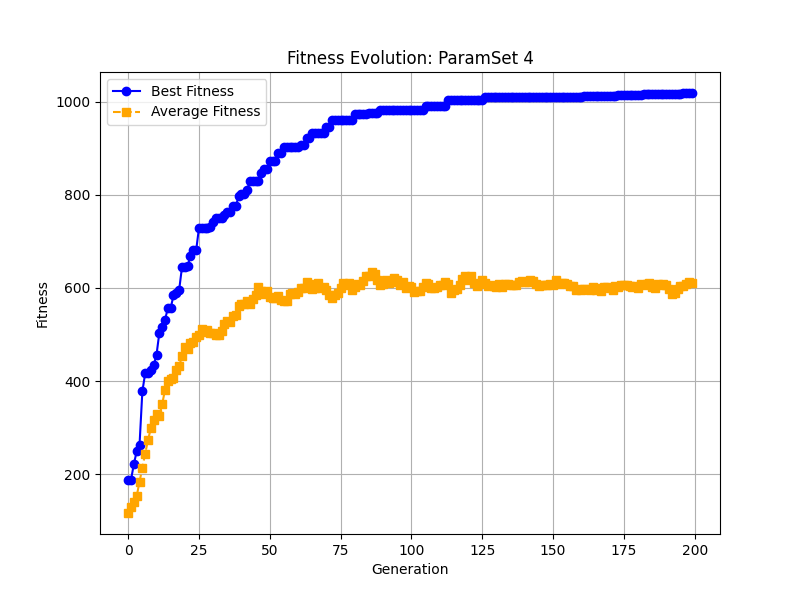
\includegraphics[width=0.3\textwidth]{img/Figure_4.png}
    \centering
    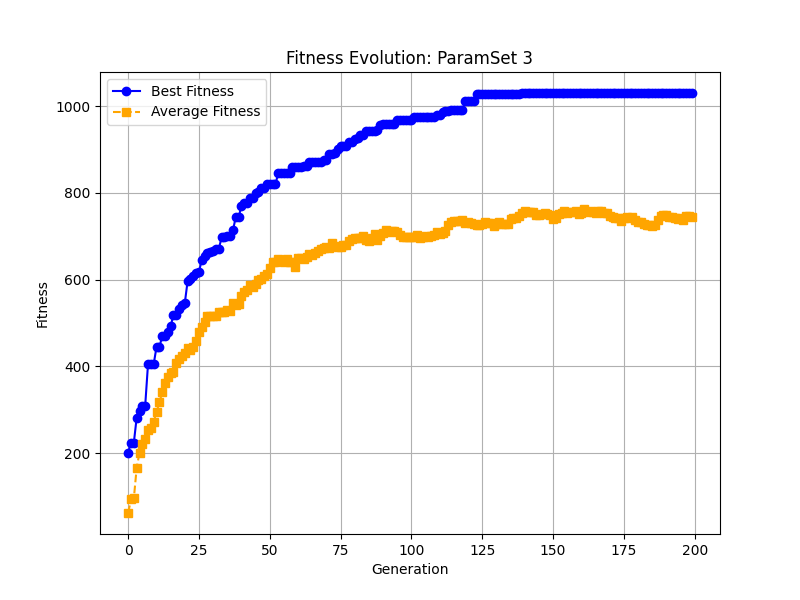
\includegraphics[width=0.3\textwidth]{img/Figure_3.png}
    \centering
    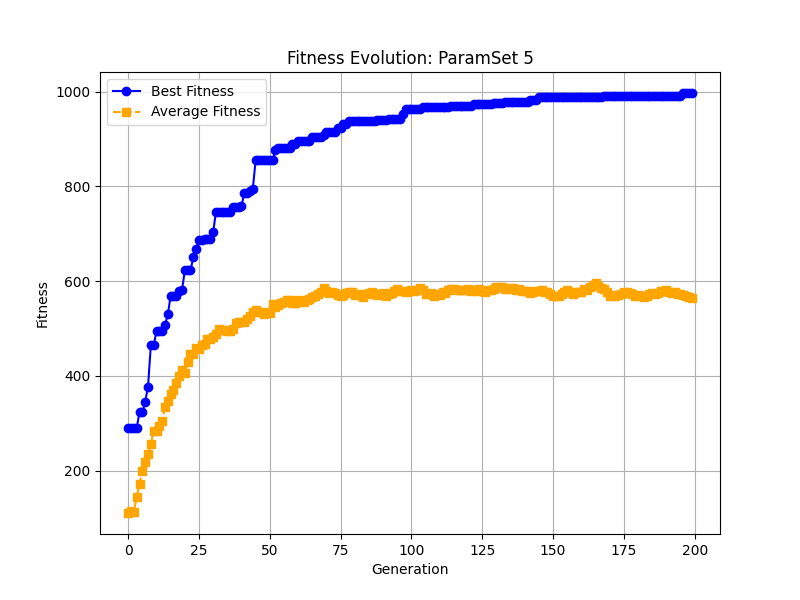
\includegraphics[width=0.3\textwidth]{img/Figure_5.png}
    \centering
    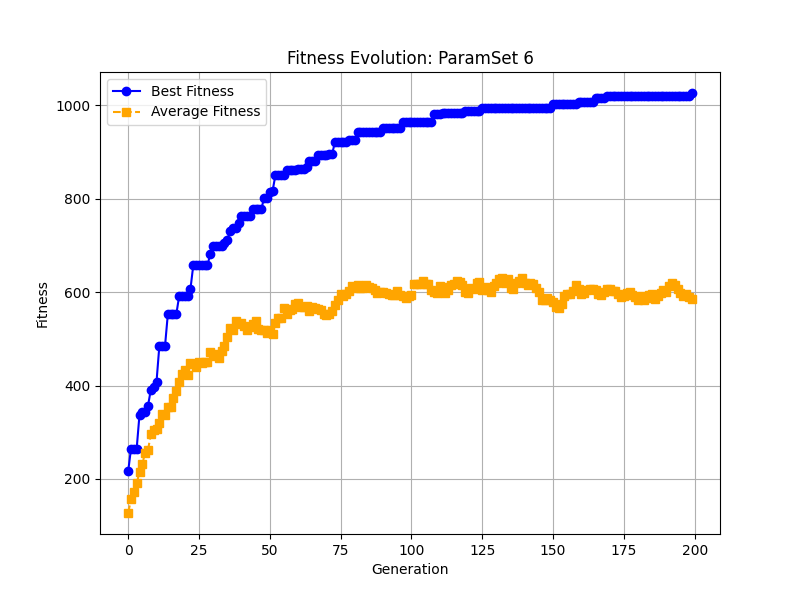
\includegraphics[width=0.3\textwidth]{img/Figure_6.png}
    \centering
    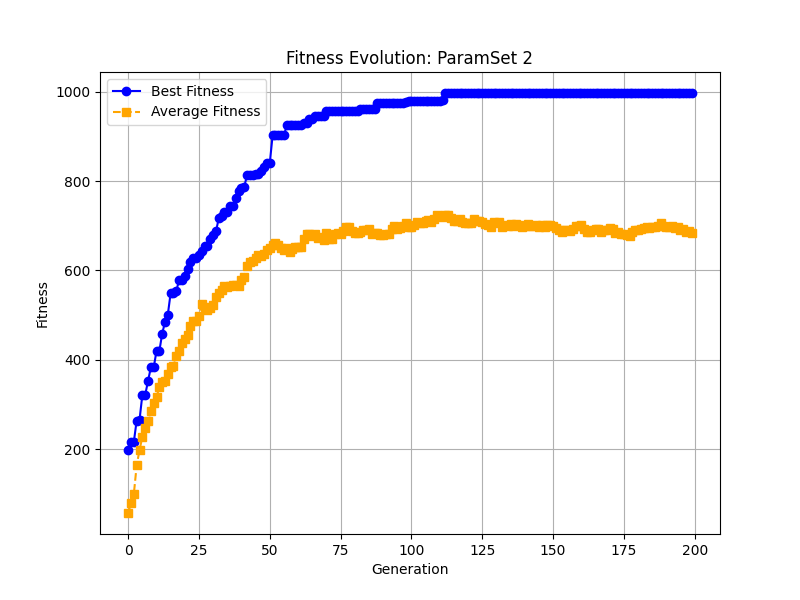
\includegraphics[width=0.3\textwidth]{img/Figure_12.png}
    \caption{遗传算法结果展示}
\end{figure}
\paragraph{整体分析}
图表展示了遗传算法运行过程中,不同参数设置下每一代的最佳适应度(蓝色曲线)和平均适应度(橙色曲线)的变化趋势。
每张子图分别对应不同的参数设置 (\texttt{ParamSet 1} 至 \texttt{ParamSet 6}),显示了在不同参数组合下算法的优化过程及性能。

\paragraph{最佳适应度的变化趋势}
\begin{itemize}
    \item \textbf{初期阶段(0-20代):}  
    所有参数设置下,最佳适应度值均快速上升。这表明遗传算法在初期能快速找到较优解,得益于精英保留和选择操作将适应度较高的个体传递至下一代。
    
    \item \textbf{中期阶段(20-100代):}  
    随着进化代数的增加,最佳适应度的增长速度逐渐减缓,曲线趋于平滑。这表明算法正在逐步收敛,高适应度解在种群中的占比不断增加。
    
    \item \textbf{后期阶段(100代以后):}  
    大部分参数设置下,最佳适应度趋于稳定,说明种群已经接近全局最优解或局部最优解,进一步提升变得困难。
\end{itemize}

\paragraph{平均适应度的变化趋势}
\begin{itemize}
    \item \textbf{初期阶段(0-20代):}  
    平均适应度曲线在初期也有显著增长,表明种群整体质量迅速提升。
    
    \item \textbf{中期阶段(20-100代):}  
    平均适应度曲线的增长速度明显减缓,曲线逐渐趋于平稳,说明种群中的解逐渐收敛至高适应度区域,种群的多样性逐渐减少。
    
    \item \textbf{后期阶段(100代以后):}  
    在后期,平均适应度曲线基本保持稳定,表明算法进入收敛状态,种群质量不再有大幅度提升。
\end{itemize}

\paragraph{参数对算法的影响}
从不同子图中可以看出,参数设置对遗传算法的表现具有显著影响:
\begin{itemize}
    \item \textbf{交叉概率 (\textit{pc}) 和变异概率 (\textit{pm}):}  
    较高的交叉概率能够更快地生成高适应度个体,而适当的变异概率有助于避免过早收敛。
    
    \item \textbf{种群规模 (\textit{P0} 和 \textit{P}):}  
    较大的种群规模能够提供更多的解空间搜索,但也可能增加计算代价。较小的种群规模容易导致算法陷入局部最优。
\end{itemize}

\paragraph{结论}
从结果来看,最佳适应度的曲线展示了算法在各参数设置下的优化能力,平均适应度曲线反映了种群整体质量的变化趋势。合理设置参数能够显著提升算法的效率与收敛性能。
\section{后文}
\paragraph{参数对算法性能的影响}
通过对六组不同参数设置的实验结果进行观察与分析,可以得出以下结论:
\begin{itemize}
    \item \textbf{交叉概率 (\textit{pc}) 的影响:}  
    高交叉概率 (\texttt{ParamSet 2, 5}) 下,最佳适应度曲线在初期阶段上升速度更快,表明交叉操作能够有效地探索解空间,快速生成高质量的后代。然而,若交叉概率过低 (\texttt{ParamSet 1}),可能导致种群的探索能力不足,影响算法效率。
    
    \item \textbf{变异概率 (\textit{pm}) 的影响:}  
    适中的变异概率 (\texttt{ParamSet 4, 5}) 能够在维持种群收敛性的同时,防止算法陷入局部最优。但若变异概率过高,可能导致种群破坏性过大,收敛变慢;而变异概率过低 (\texttt{ParamSet 1, 2}),则可能导致算法早熟收敛。
    
    \item \textbf{种群规模 (\textit{P0} 和 \textit{P}) 的影响:}  
    种群规模较大 (\texttt{ParamSet 5}) 时,算法能够更充分地探索解空间,因此曲线更加平滑且收敛效果更好。然而,过大的种群规模也会显著增加计算成本。种群规模较小 (\texttt{ParamSet 6}) 时,虽然初期收敛速度较快,但后期容易陷入局部最优。
\end{itemize}

\paragraph{最优解一致性分析}
观察每组参数的运行结果,发现不同参数设置下,最终获得的最优解并不完全一致。部分参数组合 (\texttt{ParamSet 5}) 能够更接近全局最优解,而其他组合 (\texttt{ParamSet 6}) 可能受到局部最优的限制。这表明参数设置对算法性能有显著影响,同时也体现了遗传算法的随机性。

\paragraph{实验心得}
通过本次实验,我对遗传算法的实现与优化有了更深入的理解,总结如下:
\begin{itemize}
    \item \textbf{编码设计与适应度函数的重要性:}  
    在遗传算法中,编码方式与适应度函数的设计直接决定了算法的优化方向与搜索效率。实验中,适应度函数设计为成本与收益的平衡,对于解的选择至关重要。
    
    \item \textbf{精英保留策略的作用:}  
    实验中采用了精英保留策略,有效避免了高适应度解在后代中丢失的情况。这一策略在收敛性和解的质量方面起到了重要作用。
    
    \item \textbf{参数调优的必要性:}  
    参数的选择对算法性能有显著影响。通过多组参数的实验验证,可以发现合理的参数设置(如交叉概率适中、变异概率平衡、种群规模适宜)能够显著提升算法的优化效果。
    
    \item \textbf{随机性的影响:}  
    遗传算法的运行结果具有一定随机性,即使在相同参数下,多次运行的结果也可能有所不同。因此,在实际应用中,可以通过多次实验取平均值或设置更大种群规模来提高解的可靠性。
\end{itemize}

\paragraph{总结}
本次实验展示了遗传算法在解决复杂优化问题中的有效性,同时也反映了参数设置、随机性等因素对算法性能的影响。通过合理的编码设计、适应度函数设定和参数调优,可以有效提高算法的收敛速度与解的质量。这不仅提高了我对遗传算法的理解,也让我意识到解决实际问题时需要综合考虑算法的效率和解的稳定性。
\subsection{实验分工}
\begin{itemize}
    \item 陈海弘:论文撰写排版
    \item 方唯特:实验代码编写
\end{itemize}

\end{document}
